\documentclass[a4paper]{article}

\usepackage{fullpage} % Package to use full page
\usepackage{parskip} % Package to tweak paragraph skipping
\usepackage{tikz} % Package for drawing
\usepackage{amsmath}
\usepackage{hyperref}
\usepackage{ctex}
\usepackage{amssymb}

\renewcommand\thefigure{\thesection.\arabic{figure}}
\makeatletter
\@addtoreset{figure}{section}
\makeatother

\makeatletter
\renewcommand \theequation {%
	\ifnum \c@section>\z@ \@arabic\c@section.\fi \ifnum \c@subsection>\z@
	\@arabic\c@subsection.\fi\ifnum \c@subsubsection>\z@
	\@arabic\c@subsubsection.\fi\@arabic\c@equation}
\@addtoreset{equation}{section}
\@addtoreset{equation}{subsection}
%\setcounter{section}{-1}
\makeatother

\title{最优化方法作业1}
\author{罗雁天 \\
2018310742}
\date{\today}

\begin{document}

\maketitle

\section{第一题}
\textbf{证明:}对于$\forall x^{(1)},x^{(2)}\in S$及$\forall \lambda \in [0,1]$
不妨设:
\begin{equation}
x^{(1)}=Ay^{(1)},x^{(2)}=Ay^{(2)}
\end{equation}
则:
\begin{equation}
\begin{aligned}
\lambda x^{(1)} + (1-\lambda)x^{(2)} &= \lambda A y^{(1)} + (1-\lambda) A y^{(2)} \\
&= A(\lambda y^{(1)}+(1-\lambda) y^{(2)}) 
\end{aligned}
\end{equation}
由于$y^{(1)}\ge 0,y^{(2)}\ge 0,\lambda \in [0,1]$,所以$\lambda y^{(1)}+(1-\lambda) y^{(2)}\ge 0$,

因此$\lambda x^{(1)} + (1-\lambda)x^{(2)}\in S$,所以$S$为凸集


\section{第二题}
\textbf{证明:}根据数学归纳法可以进行证明:
\begin{enumerate}
	\item 当$k=2$时,由于$x^{(1)},x^{(2)}\in S$,根据定义:
	\begin{equation}
	\sum_{i=1}^{2}\lambda_ix^{(i)}=\lambda_1x^{(1)}+(1-\lambda_1)x^{(2)} \in S
	\end{equation}
	成立
	\item 假设当$k=m$时,$\sum_{i=1}^{m}\lambda_ix^{(i)}\in S(\sum_{i=1}^{m}\lambda_{i}=1)$成立;
	
	那么当$k=m+1$时,
	\begin{equation}
	\begin{aligned}
	\sum_{i=1}^{m+1}\lambda_ix^{(i)}&=\sum_{i=1}^{m}\lambda_ix^{(i)}+\lambda_{m+1}x^{(m+1)} \\
	&=\sum_{n=1}^{m}\lambda_{n} \left( \sum_{i=1}^{m}\frac{\lambda_i}{\sum_{n=1}^{m}\lambda_{n}}x^{(i)}\right)+\lambda_{m+1}x^{(m+1)} \\
	\mbox{由于:}&\sum_{i=1}^{m}\frac{\lambda_i}{\sum_{n=1}^{m}\lambda_{n}}=1,\\
	\mbox{根据假设:}&\sum_{i=1}^{m}\frac{\lambda_i}{\sum_{n=1}^{m+1}\lambda_{n}}x^{(i)} \in S \\
	\mbox{不妨设:}&y=\sum_{i=1}^{m}\frac{\lambda_i}{\sum_{n=1}^{m}\lambda_{n}}x^{(i)} \in S \\
	\therefore \sum_{i=1}^{m+1}\lambda_ix^{(i)}&=\left(\sum_{n=1}^{m}\lambda_{n}\right) y +\lambda_{m+1}x^{(m+1)} \\
	又\because \sum_{n=1}^{m}\lambda_{n} & + \lambda_{m+1} = \sum_{n=1}^{m+1}\lambda_{n} = 1 \\
	\therefore &\sum_{i=1}^{m+1}\lambda_ix^{(i)}\in S\mbox{也成立}
	\end{aligned}
	\end{equation}
\end{enumerate}
由数学归纳法及1,2得:
\begin{equation}
\begin{aligned}
\sum_{i=1}^{k}\lambda_ix^{(i)}&\in S \\
\mbox{其中}\lambda_1+\lambda_2+\cdots+\lambda_k&=1,\lambda_{i}\ge 0,i=1,2,\cdots,k
\end{aligned}
\end{equation}

\newpage
\section{第三题}
第三题解答过程如下图\ref{image}所示
\begin{figure}[htbp]
	\centering
	\includegraphics[height=12cm]{no3.jpeg}
	\caption{\label{image}第三题解答}
\end{figure}
%\begin{figure}[!htbp]
%\begin{center}
%\begin{tikzpicture}
%\draw[domain=-1:3, color=blue] plot (\x, {2 - \x}) node[above = .5cm, right, color=blue] {$x_1+x_2=10$};
%\draw[domain=-0.3:0.2, color=red] plot(\x,10 * \x + 2) node[above = .5cm, right, color=red] {$-10x_1+x_2=10$};
%\draw[domain=-1:2, color=purple] plot (\x, {1 + \x}) node[above = .5cm, left, color=purple] {$x_1+x_2=10$};
%\draw[domain=-1:5, color=green] plot (\x, {(4 - \x)/4}) node[above = .5cm, right, color=green] {$x_1+x_2=10$};
%\draw [thick, ->] (-2,0) -- (6,0) node [above] {$x$};
%\draw [thick, ->] (0,-1) -- (0,6) node [right] {$y$};
%%\node at (.5,.75) {\textbullet};
%\end{tikzpicture}
%\end{center}
%\caption{The plot of $f(x)=1-x^2$ with a tangent at $x=.5$.}\label{exampleplot}
%\end{figure}
%\section{Introduction}
%
%Differentiation is a concept of Mathematics studied in Calculus. There is an ongoing discussion as to who was the first to define differentiation: Leibniz or Newton \cite{bardi2006calculus}.
%
%Differentiation allows for the calculation of the slope of the tangent of a curve at any given point as shown in Figure \ref{exampleplot}.
%
%\begin{figure}[!htbp]
%\begin{center}
%\begin{tikzpicture}
%\draw[domain=-2:2, color=blue] plot (\x, {1 - (\x)^2}) node[above = .5cm, right, color=blue] {$f(x)=1-x^2$};
%\draw[domain=-2:2, color=red] plot(\x,-1 * \x + 1.25) node[above = .5cm, right, color=red] {Tangent at $x=.5$};
%\draw [thick, ->] (-3,0) -- (3,0) node [above] {$x$};
%\draw [thick, ->] (0,-3) -- (0,3) node [right] {$y$};
%\node at (.5,.75) {\textbullet};
%\end{tikzpicture}
%\end{center}
%\caption{The plot of $f(x)=1-x^2$ with a tangent at $x=.5$.}\label{exampleplot}
%\end{figure}
%
%Differentiation is now a technique taught to mathematics students throughout the world. In this document I will discuss some aspects of differentiation.
%
%\section{Exploring the derivative using Sage}
%
%The definition of the limit of $f(x)$ at $x=a$ denoted as $f'(a)$ is:
%
%\begin{equation}
%f'(a) = \lim_{h\to0}\frac{f(a+h)-f(a)}{h}
%\end{equation}
%
%The following code can be used in sage to give the above limit:
%
%\begin{verbatim}
%def illustrate(f, a):
%    """
%    Function to take a function and illustrate the limiting definition of a derivative at a given point.
%    """
%    lst = []
%    for h in srange(.01, 3, .01):
%    	lst.append([h,(f(a+h)-f(a))/h])
%    return list_plot(lst, axes_labels=['$x$','$\\frac{f(%.02f+h)-f(%.02f)}{h}$' % (a,a)])
%\end{verbatim}
%
%\begin{figure}[!htbp]
%\begin{center}
%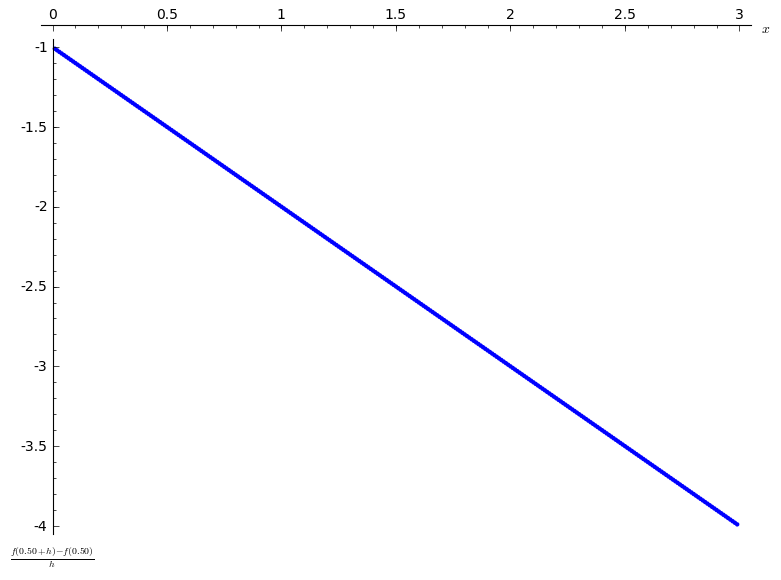
\includegraphics[width=8cm]{sage1.png}
%\end{center}
%\caption{The derivative of $f(x)=1-x^2$ at $x=.5$ converging to -1 as $h\to0$.}
%\end{figure}
%
%If we want to plot the tangent at a point $\alpha$ to a function we can use the following:
%
%\begin{align}
%y=&ax+b&&\text{(definition of a straight line)}\nonumber\\
%  &f'(a)x+b&&\text{(definition of the derivative)}\nonumber\\
%  &f'(a)x+f(a)-f'(a)a&&\text{(we know that the line intersects $f$ at $(a,f(a))$}\nonumber
%\end{align}
%
%We can combine this with the approach of the previous piece of code to see how the tangential line converges as the limiting definition of the derivative converges:
%
%\begin{verbatim}
%def convergetangentialline(f, a, x1, x2, nbrofplots=50, epsilon=.1):
%    """
%    Function to make a tangential line converge
%    """
%    clrs = rainbow(nbrofplots)
%    k = 0
%    h = epsilon
%    p = plot(f, x, x1, x2)
%    while k < nbrofplots:
%        tangent(x) = fdash(f, a, h) * x + f(a) - fdash(f, a, h) * a
%        p += plot(tangent(x), x, x1, x2, color=clrs[k])
%        h += epsilon
%        k += 1
%    return p
%\end{verbatim}
%
%The plot shown in Figure \ref{lines} shows how the lines shown converge to the actual tangent to $1-x^2$ as $x=2$ (the red line is the `closest' curve).
%
%\begin{figure}[!htbp]
%\begin{center}
%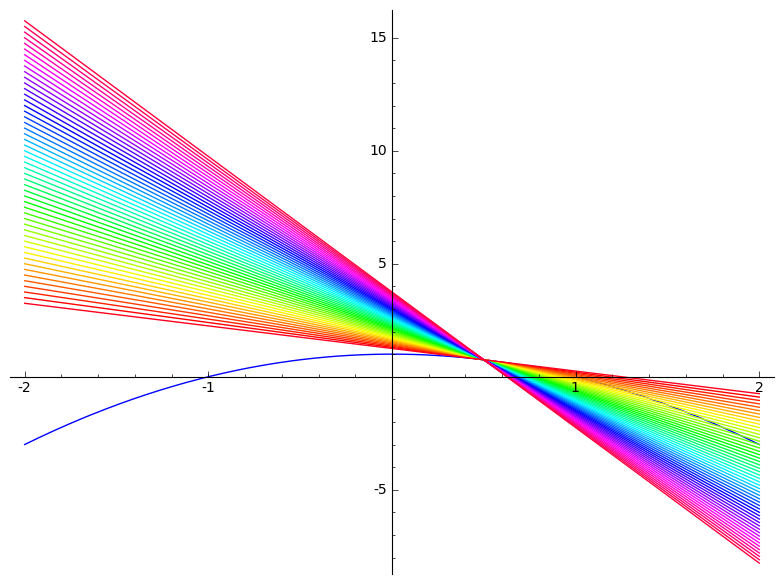
\includegraphics[width=8cm]{sage0.png}
%\end{center}
%\caption{Lines converging to the tangent curve as $h\to0$.}\label{lines}
%\end{figure}
%
%Note here that the last plot is given using the \textbf{real} definition of the derivative and not the approximation.
%
%\section{Conclusions}
%
%In this report I have explored the limiting definition of the limit showing how as $h\to 0$ we can visualise the derivative of a function. The code involved \url{https://sage.maths.cf.ac.uk/home/pub/18/} uses the differentiation capabilities of Sage but also the plotting abilities.
%
%There are various other aspects that could be explored such as symbolic differentiation rules. For example:
%
%$$\frac{dx^n}{dx}=(n+1)x^{n}\text{ if }x\ne-1$$
%
%Furthermore it is interesting to not that there exists some functions that \textbf{are not} differentiable at a point such as the function $f(x)=\sin(1/x)$ which is not differentiable at $x=0$. A plot of this function is shown in Figure \ref{notdiff}.
%
%\begin{figure}[!htbp]
%\begin{center}
%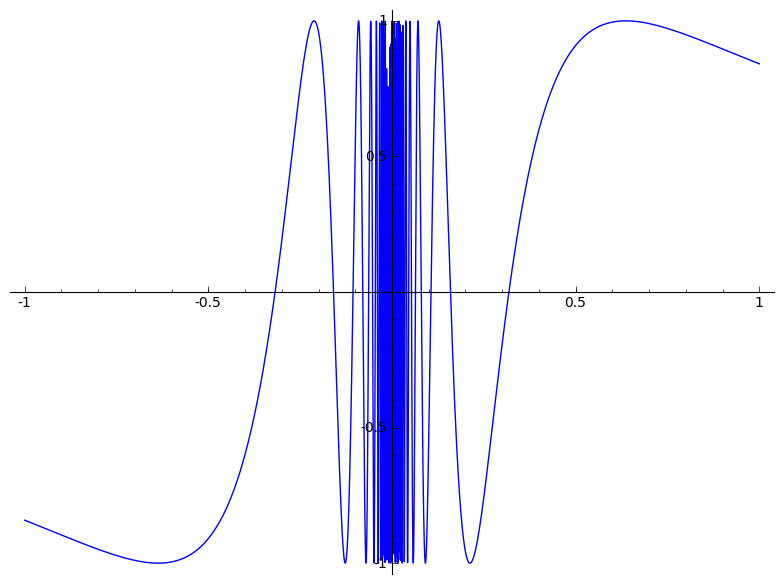
\includegraphics[width=8cm]{sage2.png}
%\end{center}
%\caption{None differentiable function at $x=0$.}\label{notdiff}
%\end{figure}
%
%
%\bibliographystyle{plain}
%\bibliography{bibliography.bib}
\end{document}